\documentclass{article}\usepackage[]{graphicx}\usepackage[]{color}
%% maxwidth is the original width if it is less than linewidth
%% otherwise use linewidth (to make sure the graphics do not exceed the margin)
\makeatletter
\def\maxwidth{ %
  \ifdim\Gin@nat@width>\linewidth
    \linewidth
  \else
    \Gin@nat@width
  \fi
}
\makeatother

\definecolor{fgcolor}{rgb}{0.345, 0.345, 0.345}
\newcommand{\hlnum}[1]{\textcolor[rgb]{0.686,0.059,0.569}{#1}}%
\newcommand{\hlstr}[1]{\textcolor[rgb]{0.192,0.494,0.8}{#1}}%
\newcommand{\hlcom}[1]{\textcolor[rgb]{0.678,0.584,0.686}{\textit{#1}}}%
\newcommand{\hlopt}[1]{\textcolor[rgb]{0,0,0}{#1}}%
\newcommand{\hlstd}[1]{\textcolor[rgb]{0.345,0.345,0.345}{#1}}%
\newcommand{\hlkwa}[1]{\textcolor[rgb]{0.161,0.373,0.58}{\textbf{#1}}}%
\newcommand{\hlkwb}[1]{\textcolor[rgb]{0.69,0.353,0.396}{#1}}%
\newcommand{\hlkwc}[1]{\textcolor[rgb]{0.333,0.667,0.333}{#1}}%
\newcommand{\hlkwd}[1]{\textcolor[rgb]{0.737,0.353,0.396}{\textbf{#1}}}%
\let\hlipl\hlkwb

\usepackage{framed}
\makeatletter
\newenvironment{kframe}{%
 \def\at@end@of@kframe{}%
 \ifinner\ifhmode%
  \def\at@end@of@kframe{\end{minipage}}%
  \begin{minipage}{\columnwidth}%
 \fi\fi%
 \def\FrameCommand##1{\hskip\@totalleftmargin \hskip-\fboxsep
 \colorbox{shadecolor}{##1}\hskip-\fboxsep
     % There is no \\@totalrightmargin, so:
     \hskip-\linewidth \hskip-\@totalleftmargin \hskip\columnwidth}%
 \MakeFramed {\advance\hsize-\width
   \@totalleftmargin\z@ \linewidth\hsize
   \@setminipage}}%
 {\par\unskip\endMakeFramed%
 \at@end@of@kframe}
\makeatother

\definecolor{shadecolor}{rgb}{.97, .97, .97}
\definecolor{messagecolor}{rgb}{0, 0, 0}
\definecolor{warningcolor}{rgb}{1, 0, 1}
\definecolor{errorcolor}{rgb}{1, 0, 0}
\newenvironment{knitrout}{}{} % an empty environment to be redefined in TeX

\usepackage{alltt}
\usepackage{url}
\usepackage{hyperref}
\usepackage{breakurl}
\usepackage{amsmath}
\usepackage{amssymb}
%\VignetteIndexEntry{Fitting and visualising row-linear models with \texttt{consensus}}
%\VignetteEngine{knitr::rmarkdown}
\IfFileExists{upquote.sty}{\usepackage{upquote}}{}
\begin{document}

\title{Fitting and visualising row-linear models with \texttt{consensus}}

\author{Tim Peters}
\maketitle

\renewcommand{\abstractname}{Summary}
\begin{abstract}
This short vignette will demonstrate how to fit a set of row-linear models in the form of an interlaboratory testing procedure (ASTM Standard E691) in a genomic context. This allows us to make comparisons of sensitivity and precision for each platform/condition the samples are measured under. We can then make broader inferences about the suitability of a given technology. 
\end{abstract}

In an ideal world we would like a set of ``gold standards'' to validate a new technology or laboratory protocol when quantifying various genomic characteristics. The problem with this is that \emph{all} genomic measurements are estimates, even those that are seen as more reliable, such as qPCR. Stochastic sampling of individual molecules (and their subsequent amplification) is an inescapable part of most modern laboratory protocols, which means that, inevitably, there will always be error present in the measurement. Rather than ignore this error and defining a ``gold standard'' (thus biasing all subsequent measurements towards that standard), the aim of this package is to encourage an empirical approach to characterising the advantages and disadvantages of a suite of candidate technological platforms, laboratory protocols or other various conditions that may influence the measurement. With this in mind, we start with some normalised gene expression data sourced from The Cancer Genome Atlas (TCGA) glioblastoma multiforme (GBM) project \cite{Verhaak}.

\begin{knitrout}
\definecolor{shadecolor}{rgb}{0.969, 0.969, 0.969}\color{fgcolor}\begin{kframe}
\begin{alltt}
\hlkwd{library}\hlstd{(rmarkdown)}
\end{alltt}
\end{kframe}
\end{knitrout}

\begin{knitrout}
\definecolor{shadecolor}{rgb}{0.969, 0.969, 0.969}\color{fgcolor}\begin{kframe}
\begin{alltt}
\hlkwd{library}\hlstd{(consensus)}
\hlkwd{data}\hlstd{(}\hlstr{"TCGA"}\hlstd{)}
\end{alltt}
\end{kframe}
\end{knitrout}

We have 27 matched samples assayed across four different gene expression measurement platforms: Affymetrix-HT-HG-U133A GeneChip,  Affymetrix HuEx GeneChip, Custom Agilent 244,000 feature Gene Expression Microarray and a polyA selection RNA-Seq protocol. We have selected 1000 genes at random for this test dataset.

\begin{knitrout}
\definecolor{shadecolor}{rgb}{0.969, 0.969, 0.969}\color{fgcolor}\begin{kframe}
\begin{alltt}
\hlstd{dims} \hlkwb{<-} \hlkwd{lapply}\hlstd{(}\hlkwd{mget}\hlstd{(}\hlkwd{ls}\hlstd{()), dim)}
\hlkwd{outer}\hlstd{(dims, dims,} \hlkwd{Vectorize}\hlstd{(all.equal))}
\end{alltt}
\begin{verbatim}
##                    Agilent                              checkMM    
## Agilent            TRUE                                 Character,3
## checkMM            "target is NULL, current is numeric" TRUE       
## fitConsensus       "target is NULL, current is numeric" TRUE       
## fitMandel          "target is NULL, current is numeric" TRUE       
## getBlock           "target is NULL, current is numeric" TRUE       
## Huex               TRUE                                 Character,3
## i                  "target is NULL, current is numeric" TRUE       
## multimeas          "target is NULL, current is numeric" TRUE       
## MultiMeasure       "target is NULL, current is numeric" TRUE       
## plotMarginals      "target is NULL, current is numeric" TRUE       
## plotMostDiscordant "target is NULL, current is numeric" TRUE       
## plotOneFit         "target is NULL, current is numeric" TRUE       
## RNASeq             TRUE                                 Character,3
## tcga_mm            "target is NULL, current is numeric" TRUE       
## U133A              TRUE                                 Character,3
##                    fitConsensus fitMandel   getBlock   
## Agilent            Character,3  Character,3 Character,3
## checkMM            TRUE         TRUE        TRUE       
## fitConsensus       TRUE         TRUE        TRUE       
## fitMandel          TRUE         TRUE        TRUE       
## getBlock           TRUE         TRUE        TRUE       
## Huex               Character,3  Character,3 Character,3
## i                  TRUE         TRUE        TRUE       
## multimeas          TRUE         TRUE        TRUE       
## MultiMeasure       TRUE         TRUE        TRUE       
## plotMarginals      TRUE         TRUE        TRUE       
## plotMostDiscordant TRUE         TRUE        TRUE       
## plotOneFit         TRUE         TRUE        TRUE       
## RNASeq             Character,3  Character,3 Character,3
## tcga_mm            TRUE         TRUE        TRUE       
## U133A              Character,3  Character,3 Character,3
##                    Huex                                 i          
## Agilent            TRUE                                 Character,3
## checkMM            "target is NULL, current is numeric" TRUE       
## fitConsensus       "target is NULL, current is numeric" TRUE       
## fitMandel          "target is NULL, current is numeric" TRUE       
## getBlock           "target is NULL, current is numeric" TRUE       
## Huex               TRUE                                 Character,3
## i                  "target is NULL, current is numeric" TRUE       
## multimeas          "target is NULL, current is numeric" TRUE       
## MultiMeasure       "target is NULL, current is numeric" TRUE       
## plotMarginals      "target is NULL, current is numeric" TRUE       
## plotMostDiscordant "target is NULL, current is numeric" TRUE       
## plotOneFit         "target is NULL, current is numeric" TRUE       
## RNASeq             TRUE                                 Character,3
## tcga_mm            "target is NULL, current is numeric" TRUE       
## U133A              TRUE                                 Character,3
##                    multimeas   MultiMeasure plotMarginals
## Agilent            Character,3 Character,3  Character,3  
## checkMM            TRUE        TRUE         TRUE         
## fitConsensus       TRUE        TRUE         TRUE         
## fitMandel          TRUE        TRUE         TRUE         
## getBlock           TRUE        TRUE         TRUE         
## Huex               Character,3 Character,3  Character,3  
## i                  TRUE        TRUE         TRUE         
## multimeas          TRUE        TRUE         TRUE         
## MultiMeasure       TRUE        TRUE         TRUE         
## plotMarginals      TRUE        TRUE         TRUE         
## plotMostDiscordant TRUE        TRUE         TRUE         
## plotOneFit         TRUE        TRUE         TRUE         
## RNASeq             Character,3 Character,3  Character,3  
## tcga_mm            TRUE        TRUE         TRUE         
## U133A              Character,3 Character,3  Character,3  
##                    plotMostDiscordant plotOneFit 
## Agilent            Character,3        Character,3
## checkMM            TRUE               TRUE       
## fitConsensus       TRUE               TRUE       
## fitMandel          TRUE               TRUE       
## getBlock           TRUE               TRUE       
## Huex               Character,3        Character,3
## i                  TRUE               TRUE       
## multimeas          TRUE               TRUE       
## MultiMeasure       TRUE               TRUE       
## plotMarginals      TRUE               TRUE       
## plotMostDiscordant TRUE               TRUE       
## plotOneFit         TRUE               TRUE       
## RNASeq             Character,3        Character,3
## tcga_mm            TRUE               TRUE       
## U133A              Character,3        Character,3
##                    RNASeq                               tcga_mm    
## Agilent            TRUE                                 Character,3
## checkMM            "target is NULL, current is numeric" TRUE       
## fitConsensus       "target is NULL, current is numeric" TRUE       
## fitMandel          "target is NULL, current is numeric" TRUE       
## getBlock           "target is NULL, current is numeric" TRUE       
## Huex               TRUE                                 Character,3
## i                  "target is NULL, current is numeric" TRUE       
## multimeas          "target is NULL, current is numeric" TRUE       
## MultiMeasure       "target is NULL, current is numeric" TRUE       
## plotMarginals      "target is NULL, current is numeric" TRUE       
## plotMostDiscordant "target is NULL, current is numeric" TRUE       
## plotOneFit         "target is NULL, current is numeric" TRUE       
## RNASeq             TRUE                                 Character,3
## tcga_mm            "target is NULL, current is numeric" TRUE       
## U133A              TRUE                                 Character,3
##                    U133A                               
## Agilent            TRUE                                
## checkMM            "target is NULL, current is numeric"
## fitConsensus       "target is NULL, current is numeric"
## fitMandel          "target is NULL, current is numeric"
## getBlock           "target is NULL, current is numeric"
## Huex               TRUE                                
## i                  "target is NULL, current is numeric"
## multimeas          "target is NULL, current is numeric"
## MultiMeasure       "target is NULL, current is numeric"
## plotMarginals      "target is NULL, current is numeric"
## plotMostDiscordant "target is NULL, current is numeric"
## plotOneFit         "target is NULL, current is numeric"
## RNASeq             TRUE                                
## tcga_mm            "target is NULL, current is numeric"
## U133A              TRUE
\end{verbatim}
\begin{alltt}
\hlkwd{rm}\hlstd{(dims)}
\hlstd{rnames} \hlkwb{<-} \hlkwd{lapply}\hlstd{(}\hlkwd{mget}\hlstd{(}\hlkwd{ls}\hlstd{()), rownames)}
\hlkwd{outer}\hlstd{(rnames, rnames,} \hlkwd{Vectorize}\hlstd{(all.equal))}
\end{alltt}
\begin{verbatim}
##                    Agilent                                checkMM    
## Agilent            TRUE                                   Character,3
## checkMM            "target is NULL, current is character" TRUE       
## fitConsensus       "target is NULL, current is character" TRUE       
## fitMandel          "target is NULL, current is character" TRUE       
## getBlock           "target is NULL, current is character" TRUE       
## Huex               TRUE                                   Character,3
## i                  "target is NULL, current is character" TRUE       
## multimeas          "target is NULL, current is character" TRUE       
## MultiMeasure       "target is NULL, current is character" TRUE       
## plotMarginals      "target is NULL, current is character" TRUE       
## plotMostDiscordant "target is NULL, current is character" TRUE       
## plotOneFit         "target is NULL, current is character" TRUE       
## RNASeq             TRUE                                   Character,3
## tcga_mm            "target is NULL, current is character" TRUE       
## U133A              TRUE                                   Character,3
##                    fitConsensus fitMandel   getBlock   
## Agilent            Character,3  Character,3 Character,3
## checkMM            TRUE         TRUE        TRUE       
## fitConsensus       TRUE         TRUE        TRUE       
## fitMandel          TRUE         TRUE        TRUE       
## getBlock           TRUE         TRUE        TRUE       
## Huex               Character,3  Character,3 Character,3
## i                  TRUE         TRUE        TRUE       
## multimeas          TRUE         TRUE        TRUE       
## MultiMeasure       TRUE         TRUE        TRUE       
## plotMarginals      TRUE         TRUE        TRUE       
## plotMostDiscordant TRUE         TRUE        TRUE       
## plotOneFit         TRUE         TRUE        TRUE       
## RNASeq             Character,3  Character,3 Character,3
## tcga_mm            TRUE         TRUE        TRUE       
## U133A              Character,3  Character,3 Character,3
##                    Huex                                   i          
## Agilent            TRUE                                   Character,3
## checkMM            "target is NULL, current is character" TRUE       
## fitConsensus       "target is NULL, current is character" TRUE       
## fitMandel          "target is NULL, current is character" TRUE       
## getBlock           "target is NULL, current is character" TRUE       
## Huex               TRUE                                   Character,3
## i                  "target is NULL, current is character" TRUE       
## multimeas          "target is NULL, current is character" TRUE       
## MultiMeasure       "target is NULL, current is character" TRUE       
## plotMarginals      "target is NULL, current is character" TRUE       
## plotMostDiscordant "target is NULL, current is character" TRUE       
## plotOneFit         "target is NULL, current is character" TRUE       
## RNASeq             TRUE                                   Character,3
## tcga_mm            "target is NULL, current is character" TRUE       
## U133A              TRUE                                   Character,3
##                    multimeas   MultiMeasure plotMarginals
## Agilent            Character,3 Character,3  Character,3  
## checkMM            TRUE        TRUE         TRUE         
## fitConsensus       TRUE        TRUE         TRUE         
## fitMandel          TRUE        TRUE         TRUE         
## getBlock           TRUE        TRUE         TRUE         
## Huex               Character,3 Character,3  Character,3  
## i                  TRUE        TRUE         TRUE         
## multimeas          TRUE        TRUE         TRUE         
## MultiMeasure       TRUE        TRUE         TRUE         
## plotMarginals      TRUE        TRUE         TRUE         
## plotMostDiscordant TRUE        TRUE         TRUE         
## plotOneFit         TRUE        TRUE         TRUE         
## RNASeq             Character,3 Character,3  Character,3  
## tcga_mm            TRUE        TRUE         TRUE         
## U133A              Character,3 Character,3  Character,3  
##                    plotMostDiscordant plotOneFit 
## Agilent            Character,3        Character,3
## checkMM            TRUE               TRUE       
## fitConsensus       TRUE               TRUE       
## fitMandel          TRUE               TRUE       
## getBlock           TRUE               TRUE       
## Huex               Character,3        Character,3
## i                  TRUE               TRUE       
## multimeas          TRUE               TRUE       
## MultiMeasure       TRUE               TRUE       
## plotMarginals      TRUE               TRUE       
## plotMostDiscordant TRUE               TRUE       
## plotOneFit         TRUE               TRUE       
## RNASeq             Character,3        Character,3
## tcga_mm            TRUE               TRUE       
## U133A              Character,3        Character,3
##                    RNASeq                                 tcga_mm    
## Agilent            TRUE                                   Character,3
## checkMM            "target is NULL, current is character" TRUE       
## fitConsensus       "target is NULL, current is character" TRUE       
## fitMandel          "target is NULL, current is character" TRUE       
## getBlock           "target is NULL, current is character" TRUE       
## Huex               TRUE                                   Character,3
## i                  "target is NULL, current is character" TRUE       
## multimeas          "target is NULL, current is character" TRUE       
## MultiMeasure       "target is NULL, current is character" TRUE       
## plotMarginals      "target is NULL, current is character" TRUE       
## plotMostDiscordant "target is NULL, current is character" TRUE       
## plotOneFit         "target is NULL, current is character" TRUE       
## RNASeq             TRUE                                   Character,3
## tcga_mm            "target is NULL, current is character" TRUE       
## U133A              TRUE                                   Character,3
##                    U133A                                 
## Agilent            TRUE                                  
## checkMM            "target is NULL, current is character"
## fitConsensus       "target is NULL, current is character"
## fitMandel          "target is NULL, current is character"
## getBlock           "target is NULL, current is character"
## Huex               TRUE                                  
## i                  "target is NULL, current is character"
## multimeas          "target is NULL, current is character"
## MultiMeasure       "target is NULL, current is character"
## plotMarginals      "target is NULL, current is character"
## plotMostDiscordant "target is NULL, current is character"
## plotOneFit         "target is NULL, current is character"
## RNASeq             TRUE                                  
## tcga_mm            "target is NULL, current is character"
## U133A              TRUE
\end{verbatim}
\begin{alltt}
\hlkwd{rm}\hlstd{(rnames)}
\hlstd{cnames} \hlkwb{<-} \hlkwd{lapply}\hlstd{(}\hlkwd{mget}\hlstd{(}\hlkwd{ls}\hlstd{()), colnames)}
\hlkwd{outer}\hlstd{(cnames, cnames,} \hlkwd{Vectorize}\hlstd{(all.equal))}
\end{alltt}
\begin{verbatim}
##                    Agilent                                checkMM    
## Agilent            TRUE                                   Character,3
## checkMM            "target is NULL, current is character" TRUE       
## fitConsensus       "target is NULL, current is character" TRUE       
## fitMandel          "target is NULL, current is character" TRUE       
## getBlock           "target is NULL, current is character" TRUE       
## Huex               TRUE                                   Character,3
## i                  "target is NULL, current is character" TRUE       
## multimeas          "target is NULL, current is character" TRUE       
## MultiMeasure       "target is NULL, current is character" TRUE       
## plotMarginals      "target is NULL, current is character" TRUE       
## plotMostDiscordant "target is NULL, current is character" TRUE       
## plotOneFit         "target is NULL, current is character" TRUE       
## RNASeq             TRUE                                   Character,3
## tcga_mm            "target is NULL, current is character" TRUE       
## U133A              TRUE                                   Character,3
##                    fitConsensus fitMandel   getBlock   
## Agilent            Character,3  Character,3 Character,3
## checkMM            TRUE         TRUE        TRUE       
## fitConsensus       TRUE         TRUE        TRUE       
## fitMandel          TRUE         TRUE        TRUE       
## getBlock           TRUE         TRUE        TRUE       
## Huex               Character,3  Character,3 Character,3
## i                  TRUE         TRUE        TRUE       
## multimeas          TRUE         TRUE        TRUE       
## MultiMeasure       TRUE         TRUE        TRUE       
## plotMarginals      TRUE         TRUE        TRUE       
## plotMostDiscordant TRUE         TRUE        TRUE       
## plotOneFit         TRUE         TRUE        TRUE       
## RNASeq             Character,3  Character,3 Character,3
## tcga_mm            TRUE         TRUE        TRUE       
## U133A              Character,3  Character,3 Character,3
##                    Huex                                   i          
## Agilent            TRUE                                   Character,3
## checkMM            "target is NULL, current is character" TRUE       
## fitConsensus       "target is NULL, current is character" TRUE       
## fitMandel          "target is NULL, current is character" TRUE       
## getBlock           "target is NULL, current is character" TRUE       
## Huex               TRUE                                   Character,3
## i                  "target is NULL, current is character" TRUE       
## multimeas          "target is NULL, current is character" TRUE       
## MultiMeasure       "target is NULL, current is character" TRUE       
## plotMarginals      "target is NULL, current is character" TRUE       
## plotMostDiscordant "target is NULL, current is character" TRUE       
## plotOneFit         "target is NULL, current is character" TRUE       
## RNASeq             TRUE                                   Character,3
## tcga_mm            "target is NULL, current is character" TRUE       
## U133A              TRUE                                   Character,3
##                    multimeas   MultiMeasure plotMarginals
## Agilent            Character,3 Character,3  Character,3  
## checkMM            TRUE        TRUE         TRUE         
## fitConsensus       TRUE        TRUE         TRUE         
## fitMandel          TRUE        TRUE         TRUE         
## getBlock           TRUE        TRUE         TRUE         
## Huex               Character,3 Character,3  Character,3  
## i                  TRUE        TRUE         TRUE         
## multimeas          TRUE        TRUE         TRUE         
## MultiMeasure       TRUE        TRUE         TRUE         
## plotMarginals      TRUE        TRUE         TRUE         
## plotMostDiscordant TRUE        TRUE         TRUE         
## plotOneFit         TRUE        TRUE         TRUE         
## RNASeq             Character,3 Character,3  Character,3  
## tcga_mm            TRUE        TRUE         TRUE         
## U133A              Character,3 Character,3  Character,3  
##                    plotMostDiscordant plotOneFit 
## Agilent            Character,3        Character,3
## checkMM            TRUE               TRUE       
## fitConsensus       TRUE               TRUE       
## fitMandel          TRUE               TRUE       
## getBlock           TRUE               TRUE       
## Huex               Character,3        Character,3
## i                  TRUE               TRUE       
## multimeas          TRUE               TRUE       
## MultiMeasure       TRUE               TRUE       
## plotMarginals      TRUE               TRUE       
## plotMostDiscordant TRUE               TRUE       
## plotOneFit         TRUE               TRUE       
## RNASeq             Character,3        Character,3
## tcga_mm            TRUE               TRUE       
## U133A              Character,3        Character,3
##                    RNASeq                                 tcga_mm    
## Agilent            TRUE                                   Character,3
## checkMM            "target is NULL, current is character" TRUE       
## fitConsensus       "target is NULL, current is character" TRUE       
## fitMandel          "target is NULL, current is character" TRUE       
## getBlock           "target is NULL, current is character" TRUE       
## Huex               TRUE                                   Character,3
## i                  "target is NULL, current is character" TRUE       
## multimeas          "target is NULL, current is character" TRUE       
## MultiMeasure       "target is NULL, current is character" TRUE       
## plotMarginals      "target is NULL, current is character" TRUE       
## plotMostDiscordant "target is NULL, current is character" TRUE       
## plotOneFit         "target is NULL, current is character" TRUE       
## RNASeq             TRUE                                   Character,3
## tcga_mm            "target is NULL, current is character" TRUE       
## U133A              TRUE                                   Character,3
##                    U133A                                 
## Agilent            TRUE                                  
## checkMM            "target is NULL, current is character"
## fitConsensus       "target is NULL, current is character"
## fitMandel          "target is NULL, current is character"
## getBlock           "target is NULL, current is character"
## Huex               TRUE                                  
## i                  "target is NULL, current is character"
## multimeas          "target is NULL, current is character"
## MultiMeasure       "target is NULL, current is character"
## plotMarginals      "target is NULL, current is character"
## plotMostDiscordant "target is NULL, current is character"
## plotOneFit         "target is NULL, current is character"
## RNASeq             TRUE                                  
## tcga_mm            "target is NULL, current is character"
## U133A              TRUE
\end{verbatim}
\begin{alltt}
\hlkwd{rm}\hlstd{(cnames)}
\end{alltt}
\end{kframe}
\end{knitrout}

Notice that the dimensions, row names and column names are identical across all measurement matrices. This is required for when we construct a MultiMeasure object from this data. If this requirement is not met, an error message will tell you which matrix attributes don't match.

Now we construct the MultiMeasure:

\begin{knitrout}
\definecolor{shadecolor}{rgb}{0.969, 0.969, 0.969}\color{fgcolor}\begin{kframe}
\begin{alltt}
\hlstd{tcga_mm} \hlkwb{<-} \hlkwd{MultiMeasure}\hlstd{(}\hlkwc{names}\hlstd{=}\hlkwd{c}\hlstd{(}\hlstr{"U133A"}\hlstd{,} \hlstr{"Huex"}\hlstd{,} \hlstr{"Agilent"}\hlstd{,} \hlstr{"RNA-Seq"}\hlstd{),}
                        \hlkwc{data}\hlstd{=}\hlkwd{list}\hlstd{(U133A, Huex, Agilent, RNASeq))}
\hlstd{tcga_mm}
\end{alltt}
\begin{verbatim}
## MultiMeasure object with 4 platforms/conditions, 27 samples and 1000 measured loci.
\end{verbatim}
\end{kframe}
\end{knitrout}

We can fit the data using the row-linear method from the ASTM standard \cite{Mandel}. One fit is performed for each gene represented by the matrix. The row-linear fit can be expressed in the form: 

\begin{equation}
Z_{ij} = a_{i} + b_{i}(x_{j} - \bar{x}) + d_{ij}
\end{equation}

where $Z_{ij}$ is 4x27 matrix of measurements from sample $j$ on platform $i$. $a_i$ is row mean of the $i$th platform, $x_j$ the column mean of the $j$th sample and $\bar{x}$ the grand mean of $Z_{ij}$. $b_i$ is the slope of the regression of the sample measurements from platform $i$ on $x_j - \bar{x}$, and $d_{ij}$ the residual scatter about this line.

Firstly, let's visualise one of these fits, from a well-known gene, TP53:

\begin{knitrout}
\definecolor{shadecolor}{rgb}{0.969, 0.969, 0.969}\color{fgcolor}\begin{kframe}
\begin{alltt}
\hlkwd{plotOneFit}\hlstd{(tcga_mm,} \hlstr{"TP53"}\hlstd{,} \hlkwd{brewer.pal}\hlstd{(}\hlkwc{n} \hlstd{=} \hlnum{4}\hlstd{,} \hlkwc{name} \hlstd{=} \hlstr{"Dark2"}\hlstd{))}
\end{alltt}
\end{kframe}
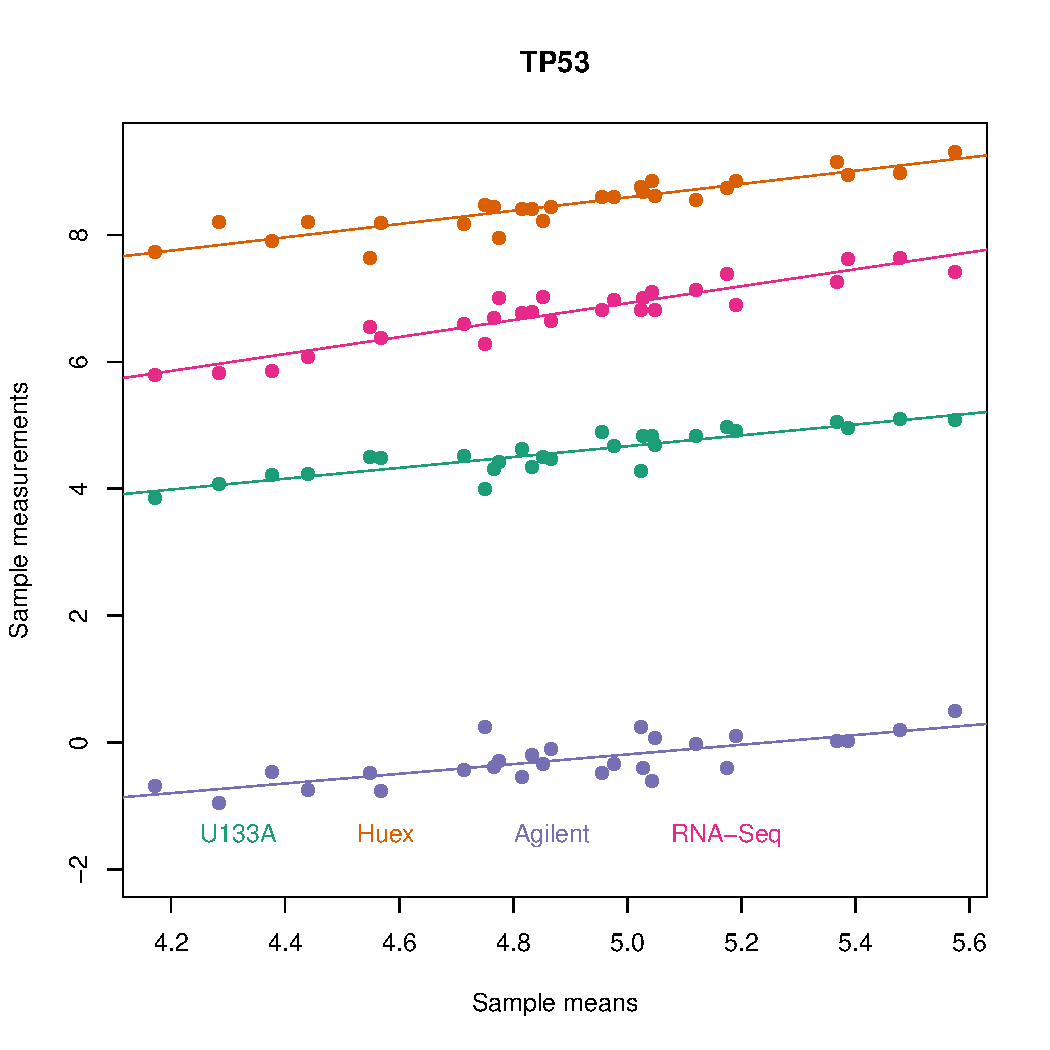
\includegraphics[width=\maxwidth]{figure/tp53-1} 

\end{knitrout}

This gene is generally concordant across platforms, since the regression lines are fairly parallel and the residuals don't fall too far away.

Now to perform the fitting. This will create a S4 class object of type ConsensusFit.

\begin{knitrout}
\definecolor{shadecolor}{rgb}{0.969, 0.969, 0.969}\color{fgcolor}\begin{kframe}
\begin{alltt}
\hlstd{fit} \hlkwb{<-} \hlkwd{fitConsensus}\hlstd{(tcga_mm)}
\end{alltt}


{\ttfamily\noindent\bfseries\color{errorcolor}{\#\# Error in rowVars(a\_i): could not find function "{}rowVars"{}}}\begin{alltt}
\hlstd{fit}
\end{alltt}


{\ttfamily\noindent\bfseries\color{errorcolor}{\#\# Error in eval(expr, envir, enclos): object 'fit' not found}}\end{kframe}
\end{knitrout}

Once this is done, we might be interested in seeing what the distributions of some parameters from Equation (1) look like over all 1000 genes. First, let's see what the distribution of the averages ($a_i$s) are, which serve as dynamic ranges of each platform:

\begin{knitrout}
\definecolor{shadecolor}{rgb}{0.969, 0.969, 0.969}\color{fgcolor}\begin{kframe}
\begin{alltt}
\hlkwd{plotMarginals}\hlstd{(fit,} \hlstr{"average"}\hlstd{,} \hlkwd{brewer.pal}\hlstd{(}\hlkwc{n} \hlstd{=} \hlnum{4}\hlstd{,} \hlkwc{name} \hlstd{=} \hlstr{"Dark2"}\hlstd{))}
\end{alltt}


{\ttfamily\noindent\bfseries\color{errorcolor}{\#\# Error in class(consfit) == "{}ConsensusFit"{}: object 'fit' not found}}\end{kframe}
\end{knitrout}

Then we can see which platforms have the greatest sensitivity ($b_i$) to changes in gene expression:

\begin{knitrout}
\definecolor{shadecolor}{rgb}{0.969, 0.969, 0.969}\color{fgcolor}\begin{kframe}
\begin{alltt}
\hlkwd{plotMarginals}\hlstd{(fit,} \hlstr{"sensitivity"}\hlstd{,} \hlkwd{brewer.pal}\hlstd{(}\hlkwc{n} \hlstd{=} \hlnum{4}\hlstd{,} \hlkwc{name} \hlstd{=} \hlstr{"Dark2"}\hlstd{))}
\end{alltt}


{\ttfamily\noindent\bfseries\color{errorcolor}{\#\# Error in class(consfit) == "{}ConsensusFit"{}: object 'fit' not found}}\end{kframe}
\end{knitrout}

Clearly, RNA-Seq is the most sensitive, followed by the Agilent array, then Huex and finally U133A. Interestingly, U133A has a second mode at 0, which is indicative of a subset of genes that do not show any response to expression change on this platform. The marginals of the averages for this platform show a right skew, which contributes to this phenomenon. 

Let's plot the precision ($d_i$) marginals, remembering that higher values mean lower precision:

\begin{knitrout}
\definecolor{shadecolor}{rgb}{0.969, 0.969, 0.969}\color{fgcolor}\begin{kframe}
\begin{alltt}
\hlkwd{plotMarginals}\hlstd{(fit,} \hlstr{"precision"}\hlstd{,} \hlkwd{brewer.pal}\hlstd{(}\hlkwc{n} \hlstd{=} \hlnum{4}\hlstd{,} \hlkwc{name} \hlstd{=} \hlstr{"Dark2"}\hlstd{))}
\end{alltt}


{\ttfamily\noindent\bfseries\color{errorcolor}{\#\# Error in class(consfit) == "{}ConsensusFit"{}: object 'fit' not found}}\end{kframe}
\end{knitrout}

All platforms except U133A are generally similar in their precision, suggesting that, from a platform design perspective, there may have been a trade-off between risk and reward in detecting changes in gene expression on U133A that has now been surmounted by more recent technologies.

Finally, we are interested in the gene loci whose measurements are the most \emph{dis}cordant across platforms. These are most easily visualised on a heatmap. Like with \texttt{plotMarginals}, we can choose to plot discordance in terms of average, sensitivity or precision.

\begin{knitrout}
\definecolor{shadecolor}{rgb}{0.969, 0.969, 0.969}\color{fgcolor}\begin{kframe}
\begin{alltt}
\hlkwd{plotMostDiscordant}\hlstd{(fit,} \hlstr{"sensitivity"}\hlstd{,} \hlnum{15}\hlstd{)}
\end{alltt}


{\ttfamily\noindent\bfseries\color{errorcolor}{\#\# Error in class(consfit) == "{}ConsensusFit"{}: object 'fit' not found}}\end{kframe}
\end{knitrout}

Clearly, the governing feature of the most sensitivity-discordant genes is that RNA-Seq explains the vast majority of change in gene expression. To see what a row-linear fit looks like for one of these genes, we again use \texttt{plotOneFit}. 

\begin{knitrout}
\definecolor{shadecolor}{rgb}{0.969, 0.969, 0.969}\color{fgcolor}\begin{kframe}
\begin{alltt}
\hlkwd{plotOneFit}\hlstd{(tcga_mm,} \hlstr{"MYO7B"}\hlstd{,} \hlkwd{brewer.pal}\hlstd{(}\hlkwc{n} \hlstd{=} \hlnum{4}\hlstd{,} \hlkwc{name} \hlstd{=} \hlstr{"Dark2"}\hlstd{))}
\end{alltt}
\end{kframe}
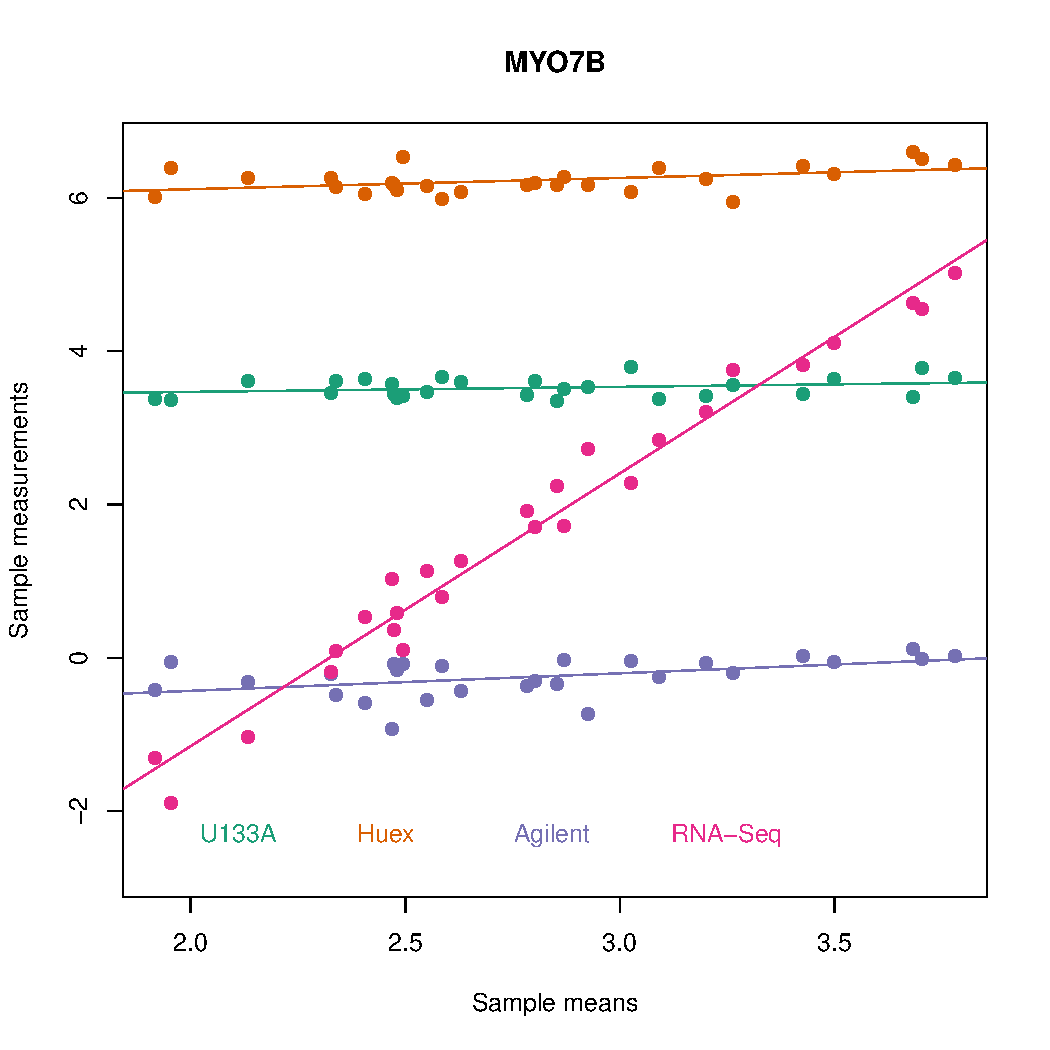
\includegraphics[width=\maxwidth]{figure/my07b-1} 

\end{knitrout}

\begin{knitrout}
\definecolor{shadecolor}{rgb}{0.969, 0.969, 0.969}\color{fgcolor}\begin{kframe}
\begin{alltt}
\hlkwd{sessionInfo}\hlstd{()}
\end{alltt}
\begin{verbatim}
## R version 3.5.0 (2018-04-23)
## Platform: x86_64-pc-linux-gnu (64-bit)
## Running under: Ubuntu 16.04.4 LTS
## 
## Matrix products: default
## BLAS: /home/timpet/R/x86_64-pc-linux-gnu-library/R-3.5.0/lib/libRblas.so
## LAPACK: /home/timpet/R/x86_64-pc-linux-gnu-library/R-3.5.0/lib/libRlapack.so
## 
## locale:
##  [1] LC_CTYPE=en_AU.UTF-8       LC_NUMERIC=C              
##  [3] LC_TIME=en_AU.UTF-8        LC_COLLATE=en_AU.UTF-8    
##  [5] LC_MONETARY=en_AU.UTF-8    LC_MESSAGES=en_AU.UTF-8   
##  [7] LC_PAPER=en_AU.UTF-8       LC_NAME=C                 
##  [9] LC_ADDRESS=C               LC_TELEPHONE=C            
## [11] LC_MEASUREMENT=en_AU.UTF-8 LC_IDENTIFICATION=C       
## 
## attached base packages:
## [1] stats     graphics  grDevices utils     datasets  methods   base     
## 
## other attached packages:
## [1] consensus_0.99.4     rmarkdown_1.9        knitr_1.20          
## [4] BiocCheck_1.16.0     RColorBrewer_1.1-2   BiocInstaller_1.30.0
## 
## loaded via a namespace (and not attached):
##  [1] Rcpp_0.12.16        compiler_3.5.0      highr_0.6          
##  [4] bitops_1.0-6        tools_3.5.0         digest_0.6.15      
##  [7] evaluate_0.10.1     graph_1.58.0        yaml_2.1.19        
## [10] parallel_3.5.0      httr_1.3.1          stringr_1.3.1      
## [13] gtools_3.5.0        caTools_1.17.1      stats4_3.5.0       
## [16] rprojroot_1.3-2     getopt_1.20.2       optparse_1.4.4     
## [19] Biobase_2.40.0      R6_2.2.2            XML_3.98-1.11      
## [22] RBGL_1.56.0         gdata_2.18.0        magrittr_1.5       
## [25] backports_1.1.2     gplots_3.0.1        codetools_0.2-15   
## [28] htmltools_0.3.6     matrixStats_0.53.1  biocViews_1.48.0   
## [31] BiocGenerics_0.26.0 stringdist_0.9.4.7  RUnit_0.4.31       
## [34] KernSmooth_2.23-15  stringi_1.2.2       RCurl_1.95-4.10
\end{verbatim}
\end{kframe}
\end{knitrout}

\begin{thebibliography}{9}

\bibitem{Verhaak}
  Verhaak, R. G. W., Hoadley, K. A., Purdom, E., Wang, V., Qi, Y., Wilkerson, M. D., ..., Cancer Genome Atlas Research Network. Integrated genomic analysis identifies clinically relevant subtypes of glioblastoma characterized by abnormalities in PDGFRA, IDH1, EGFR, and NF1. \emph{Cancer Cell}, 2010, \textbf{17}(1), 98-110. 
  
\bibitem{Mandel}
Mandel, J. Analyzing Interlaboratory Data According to ASTM Standard E691. In \emph{Quality and Statistics: Total Quality Management} (pp. 59-59-12), 1994. 100 Barr Harbor Drive, PO Box C700, West Conshohocken, PA 19428-2959: ASTM International.

\end{thebibliography}


\end{document}
